\documentclass{article}

\usepackage[utf8]{inputenc}
\usepackage[brazilian]{babel}
\usepackage{graphicx}
\usepackage{float}
\usepackage[pdftex]{hyperref}
\usepackage{epstopdf}
\usepackage{etoolbox}
\usepackage{amsmath}
\usepackage{amsfonts}
\usepackage{amssymb}
\usepackage{caption}
\usepackage{subcaption}
\usepackage{setspace}
\usepackage{tikz}

\patchcmd{\thebibliography}{\section*}{\section}{}{}
\newcommand{\R}{\ensuremath{\mathbb{R}}}
\newcommand{\Prob}{\ensuremath{\mathbb{P}}}
\newcommand{\K}{\ensuremath{\mathbb{K}}}
\newcommand{\U}{\ensuremath{\mathbb{U}}}
\newcommand{\N}{\ensuremath{\mathbb{N}}}
\newcommand{\Lg}{\ensuremath{\mathbb{L}}}
\newcommand{\T}{\ensuremath{\rm Tr}}
\newcommand{\sg}{{\sigma(x_k)}}

\newcommand{\G}{\ensuremath{\mathcal{G}}}
\newcommand{\F}{\ensuremath{\mathcal{F}}}
\newcommand{\C}{\ensuremath{\mathcal{C}}}
\newcommand{\E}{\ensuremath{\mathcal{E}}}
\newcommand{\Hn}{\ensuremath{\mathcal{H}}}
%\newcommand{\Hoo}{\ensuremath{\mathcal{H}_\infty}}
\newcommand{\Hop}{\ensuremath{\mathcal{H}_{op}}}
% --------------------------------------------------
\newtheorem{theo}{Teorema}
\newtheorem{exa}{Exemplo}
\newtheorem{lemm}{Lema}
\newtheorem{coro}{Corolário}
\newtheorem{defn}{Definição}[section]

%opening


\begin{document}
\input{capa.tex}

\onehalfspacing
\section{Objetivos} 
O objetivo desse experimento é a familiarização com o projeto e a implementação de controladores PID analógicos utilizando resistores, capacitores e amplificadores operacionais e a comparação de seu desempenho com controladores discretos. 
	
\section{Projeto do Controlador Analógico}
Consideramos a planta cuja função de transferência é representada pela equação \ref{eq:gs}, que foi obtida seguindo o método apresentado no experimento 2 \cite{bb:lab2}, consideramos também o controlador PID do experimento 3 obtido com o auxílio da ferramenta SISOTool do Matlab, cuja função vemos na equação \ref{eq:pids}.\\

\begin{equation}
\label{eq:gs}
G(s) = \frac{\kappa_1*\kappa_2*\kappa_3*\kappa_4}{(s*\tau_2 + 1)(s*\tau_3 + 1)s}
\end{equation}

\begin{table}[H]
\centering
\caption{Parâmetros numéricos da função de transferência}
\label{tab:valores}
\begin{tabular}{|c|c|}
	\hline Componente & Valor \\ 
	\hline $\kappa_1$ & $-0.1005$\\ 
	\hline $\kappa_2$ & $-2.1508$\\ 
	\hline $\kappa_3$ & $-4.6448$\\ 
	\hline $\kappa_4$ & $-5.6307$\\ 
	\hline $\tau_2$ & $0.0210$\\ 
	\hline $\tau_3$ & $0.0244$ \\ 	
	\hline 
\end{tabular} 
\end{table}

\begin{equation}
\label{eq:pidz}
K_z(s) = 9.05+\frac{142}{s}+0.144 s
\end{equation}

\begin{equation}
\label{eq:pids}
K_s(s) = 5.3+\frac{2.37}{s}+0.207 s
\end{equation}

Por fim consideramos também o controlador proposto no pré relatório \cite{bb:prelab4} que se aproxima do controlador obtido com o auxílio do SISOTool.
Utilizando o modelo proposto no roteiro \cite{bb:roteiro} mostrado na figura \ref{fig:circuito}. Com a aproximação mostrada na equação \ref{eq:kpkikd}, podemos determinar os valores de $R_1$, $R_2$ e $R_3$ dado que foi fixado $C=1 \mu F$ para obter os desejados valores de $\kappa_p$, $\kappa_i$ e $\kappa_d$.

\begin{figure}[H]
	\centering
	\includegraphics[width=\linewidth]{circuito}
	\caption{Circuito analógico para controlador PID}
	\label{fig:circuito}
\end{figure}

\begin{equation}
\label{eq:kpkikd}
\frac{\kappa_d s^2+\kappa_p s+\kappa_i}{s} \approx \frac{\frac{R_1 R_3 C}{R_1 + R_2} s^2 + \frac{R_1 + R_3}{R_1 + R_2} s+\frac{1}{R_1 + R_2}}{\frac{R_1 R_2 C}{R_1 + R_2}s^2 +s} 
\end{equation}

Encontramos então, conforme descrito no pré relatório \cite{bb:prelab4}, os valores $R_1=51k\Omega$, $R_2=1.5k\Omega$ e $R_3=200k\Omega$. E o controlador representado pela equação \ref{eq:pida}
\begin{equation}
\label{eq:pida}
K_a(s) = 4.78 + \frac{19.05}{s} + 0.194 s
\end{equation}
\section{Análise dos Resultados}
Seguindo a metodologia descrita no roteiro \cite{bb:roteiro}, implementamos o sistema planta-controlador analógico e medimos sua resposta a uma onda quadrada de amplitude de $1V$ e frequência de $0.25Hz$ com o auxílio do LabView e da plataforma de desenvolvimento Elvis. Podemos ver que o esforço de controle apresenta um pico no momento das transições, esse pico se deve principalmente à ação do termo derivativo do controlador, uma vez que nas transições a derivada da entrada é infinita, porém, ainda assim, o mesmo se mantém dentro dos $10V$ aceitáveis.

\begin{figure}[H]
	\centering
	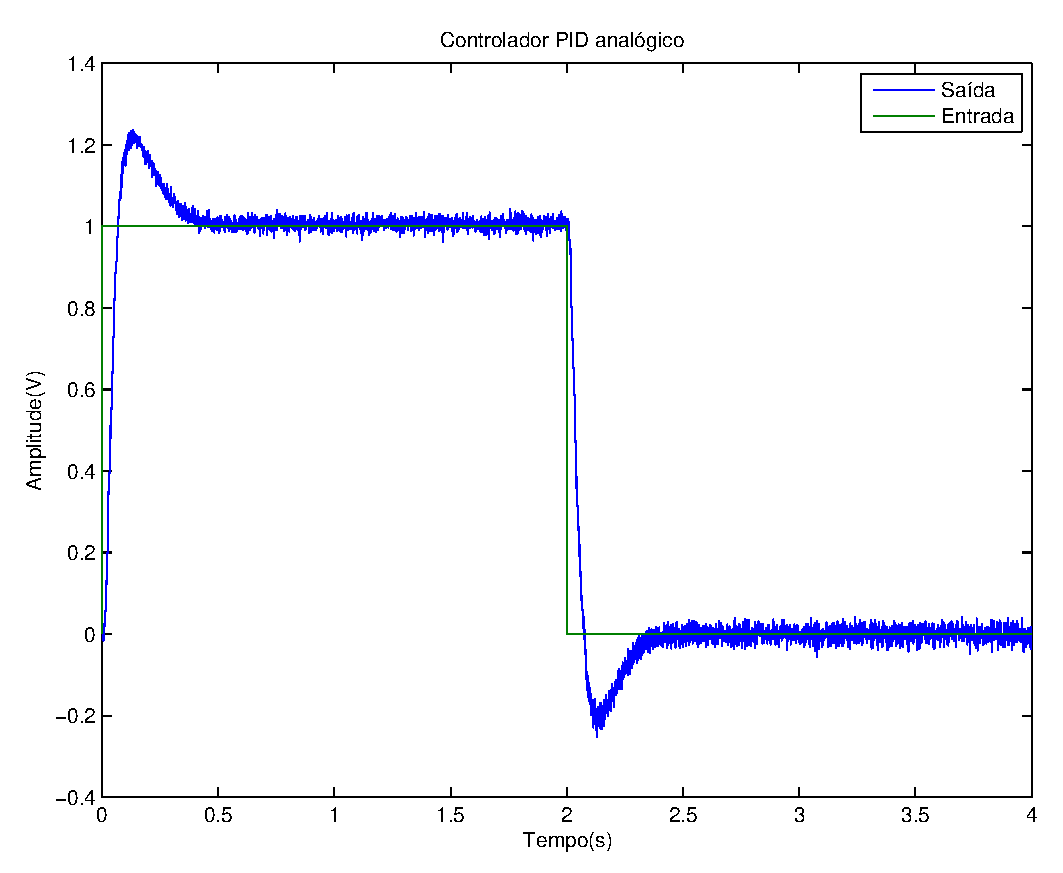
\includegraphics[width=0.8\linewidth]{ysemfiltro}
	\caption{Resposta do controlador PID analógico para onda quadrada}
	\label{fig:ysemfiltro}
\end{figure}
\begin{figure}[H]
	\centering
	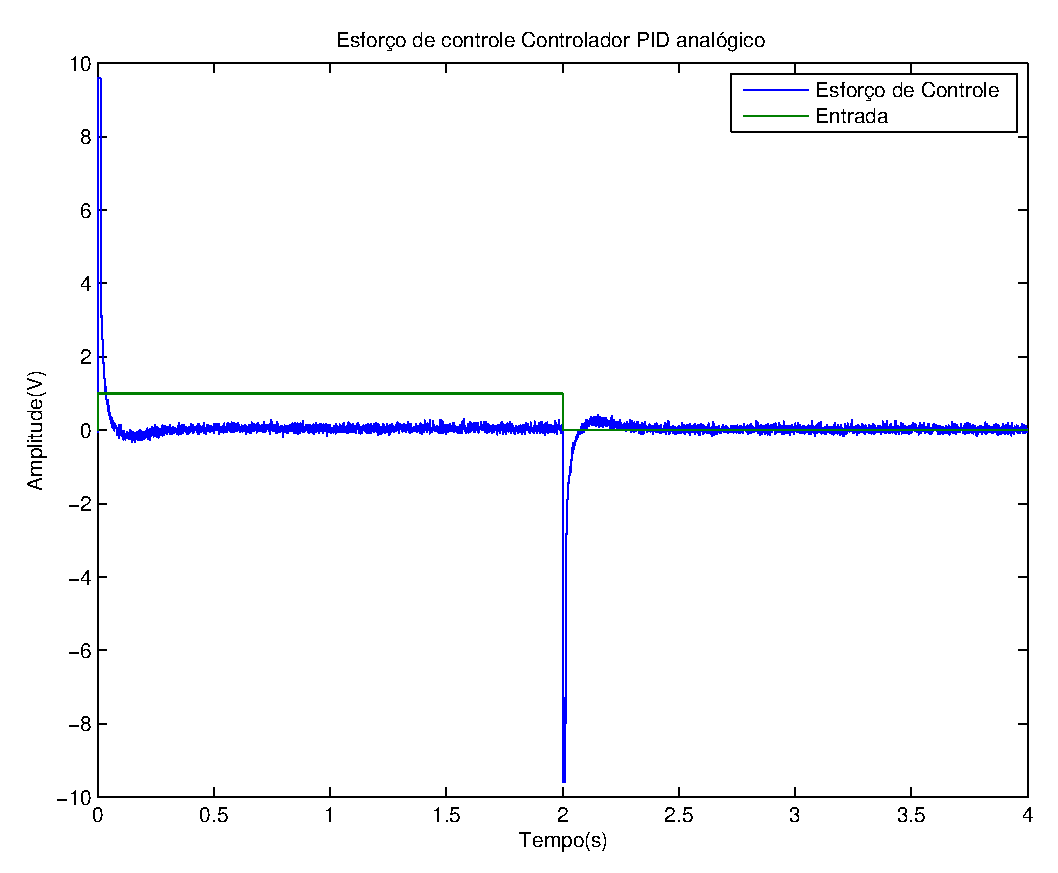
\includegraphics[width=0.8\linewidth]{upid}
	\caption{Esforço de controle do controlador PID analógico para onda quadrada}
	\label{fig:upid}
\end{figure}

Com o auxílio da função \textit{stepinfo} do Matlab obtivemos alguns indicadores de desempenho para esse controlador, após filtrar a saída para eliminar os ruídos, que estão apresentados na tabela \ref{tab:pida}
\begin{table}[H]
	\centering
	\caption{Indicadores de desempenho para controlador PID analógico}
	\label{tab:pida}
	\begin{tabular}{|c|c|}
		\hline Indicador & Valor \\ 
		\hline Tempo de subida & $0.0426s$\\ 
		\hline Tempo de estabilização & $0.4049s$\\ 
		\hline Sobrelevação & $21.9079\%$\\ 
		\hline Erro estacionário& $0.003 V$\\ 
		\hline 
	\end{tabular} 
\end{table}

\section{Comparação com PID Simulado}
Durante as simulações realizadas para o pré roteiro \cite{bb:prelab4} nós encontramos os valores apresentados na tabela \ref{tab:pidsim}.\\
\begin{table}[H]
	\centering
	\caption{Indicadores de desempenho para controlador PID analógico simulado}
	\label{tab:pidsim}
	\begin{tabular}{|c|c|}
		\hline Indicador & Valor \\ 
		\hline Tempo de subida & $0.1037s$\\ 
		\hline Tempo de estabilização & $0.7430s$\\ 
		\hline Sobrelevação & $19.0416\%$\\ 
		\hline Erro estacionário& $0V$\\ 
		\hline 
	\end{tabular} 
\end{table}
Como podemos ver o PID simulado apresenta um desempenho relativamente pior do que o implementado, seu tempo de estabilização é praticamente o dobro, enquanto sua sobrelevação é inferior em somente $2.8 \%$ da sobrelevação apresentada pelo sistema físico. Essas diferenças são mais notáveis ao comparar as duas respostas (após filtrar a saída do sistema físico) como mostrado na figura \ref{fig:yrsim}.
\begin{figure}[H]
	\centering
	\includegraphics[width=0.8\linewidth]{yrsim}
	\caption{Respostas dos controladores PID analógicos físico e simulado para onda quadrada}
	\label{fig:yrsim}
\end{figure}
Acreditamos que essas diferenças se dão, em grande parte, porque o sistema simulado não é realmente analógico, tendo passado por uma discretização durante a simulação, e do fato da planta calculada diferir da planta física.

Podemos ver também diferenças notáveis no esforço de controle dos dois controladores, como pode ser visto na figura \ref{fig:ursim}. Durante a simulação nós obtivemos picos de tensão altíssimos nas transições, notavelmente devido à ação do termo derivativo do controlador, uma vez que durante as transições de uma onda quadrada a derivada da função tende ao infinito. Porém no sistema real essas mesmas transições ficaram limitadas as proximidades dos $10V$. Isso acontece provavelmente pois no sistema real, as transições da onda são mais suaves por limitações físicas do sistema.
\begin{figure}[H]
	\centering
	\includegraphics[width=0.8\linewidth]{ursim}
	\caption{Esforços de controle dos controladores PID analógicos físico e simulado para onda quadrada}
	\label{fig:ursim}
\end{figure}

Por fim, mostramos uma comparação entre o resultado deste controlador analógico e o do controlador digital no qual ele foi inspirado, vistos na figura \ref{fig:yad}. Podemos notar que na sua versão digital, o sistema não chegou nem mesmo à se estabilizar. Parte da diferença entre os dois sistemas está no aumento significativo do termo integral do controlador, porém esse termo também aumentaria as oscilações do sistema, não sendo capaz de trazer o mesmo para a estabilidade sozinho. Acreditamos que por ser menos influenciado pelos ruídos de medida o controlador analógico apresentou um desempenho significativamente melhor, corroborando com a análise feita durante o relatório do experimento 3 \cite{bb:lab3}.
\begin{figure}[H]
	\centering
	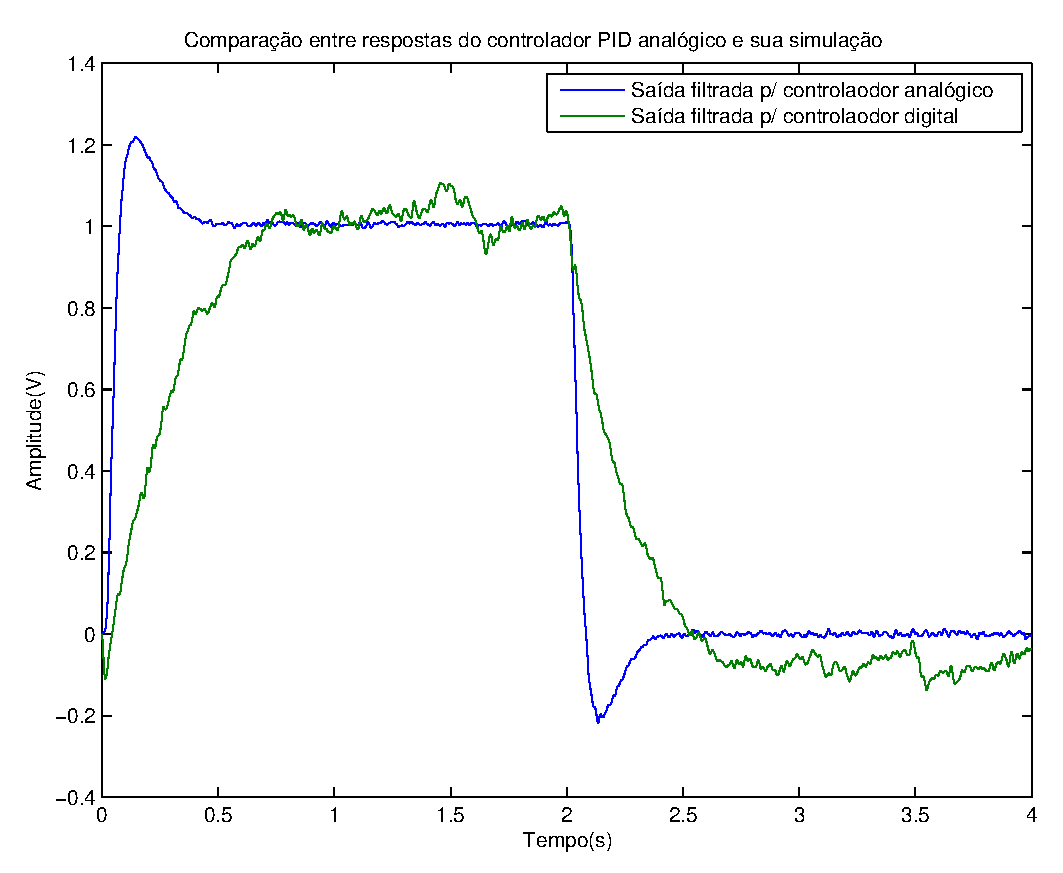
\includegraphics[width=0.8\linewidth]{yad}
	\caption{Respostas dos controladores PID analógico e digital para onda quadrada}
	\label{fig:yad}
\end{figure}

\begin{thebibliography}{widestlabel}
	\bibitem{bb:roteiro}{Roteiro do experimento disponibilizado para os alunos}
	\bibitem{bb:lab2}{KIAN, Marcelli; OLIVEIRA, Daniel. \textit{Relatório - Experimento 2:} Identificação de plantas eletrônicas.}
	\bibitem{bb:lab3}{KIAN, Marcelli; OLIVEIRA, Daniel. \textit{Relatório - Experimento 3:} Controle de plantas eletrônicas utilizando um controlador PID digital.}
	\bibitem{bb:prelab4}{KIAN, Marcelli; OLIVEIRA, Daniel. \textit{Pré Relatório - Experimento 4:}  Controle de plantas eletrônicas utilizando um controlador PID analógico.}
\end{thebibliography}
\end{document}

